\documentclass[a4paper, 12pt]{article}

\usepackage[ngerman]{babel}
\usepackage[T1]{fontenc}
\usepackage{amsmath}
\usepackage{graphicx}
\usepackage{hyperref}

\usepackage[a4paper,
            bindingoffset=0.2in,
            left=1cm,
            right=1cm,
            top=1in,
            bottom=1in,
            footskip=.25in]{geometry}
            
\title{Pre-LAB: Pendel, Team 4}
\author{Justus Weyers, Milena Mensching}
\begin{document}
\maketitle

\section{Arten von optischen Linsen}
\textbf{Welche Art von Linsen bündeln bzw. zerstreuen einfallende Lichtstrahlen?}
\begin{itemize}
	\item Bündeln: Konvexlinse
	\item Zerstreuen: Konkavlinse
\end{itemize}

\section{Reelle und virtuelle Bider}
\textbf{Was versteht man unter reellen bzw. virtuellen Bildern?}

Bei Reellen Bildern gehen vom Bild Lichtstrahlen aus. 
Diese Bilder sind auf einem Schirm abbildbar. Bei virtuellen Bildern geht von dem Bild kein Licht aus, diese sind nicht auf einem Schirm abbildbar. 
Beispiel hierfür sind ebene Spiegel, in denen ein Spiegelbild eines Objektes zu sehen ist. 
Dort wo sich das Bild zu befinden scheint, also auf der Rückseite des Spiegels, gibt es allerdings keine Lichtstrahlen.
\vspace*{0.66cm}

\textbf{Für welche Gegenstandsweiten erscheint ein virtuelles Bild bzw. ein reelles Bild? Bei welchen erscheint ein reelles Bild vergrößert oder verkleinert? 
Fertigen Sie hierzu bitte jeweils eine schematische Skizze an, die den Strahlengang an einer Sammellinse verdeutlicht.}
\begin{figure}[h]
\centering
	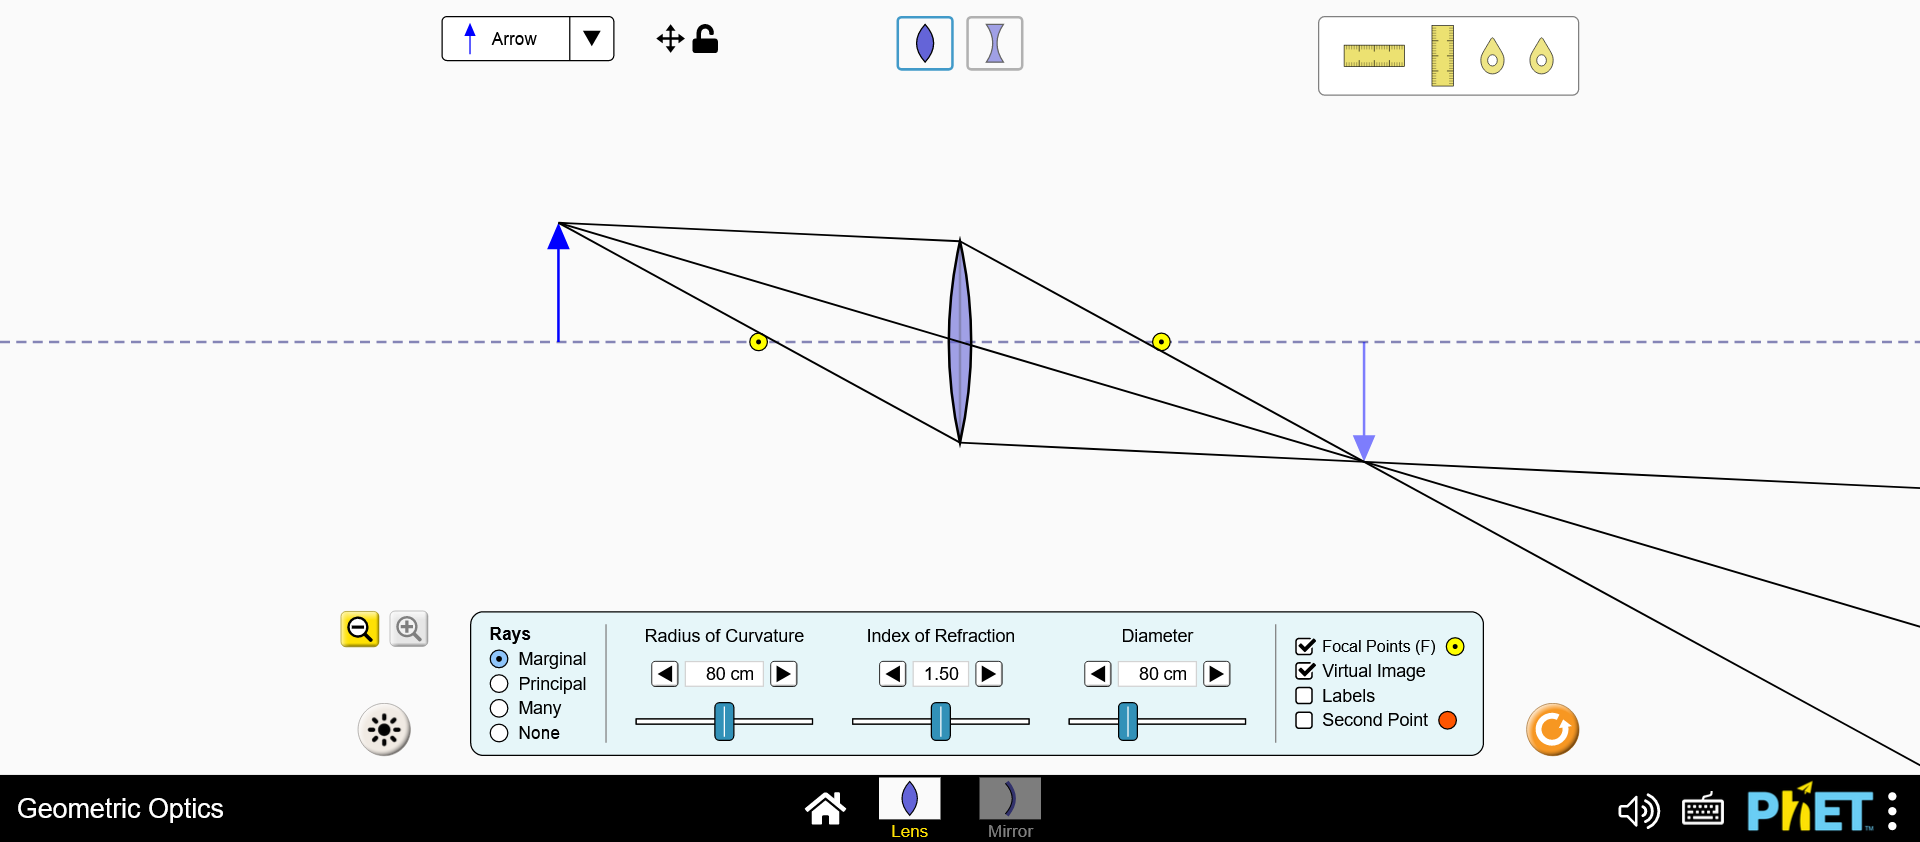
\includegraphics[scale=0.28]{A.png}
	\caption{Ein reelles Bild entsteht, wenn die Gegenstandsweite größer als die Brennweite der Linse ist.}
\end{figure}
\begin{figure}[h]
\centering
	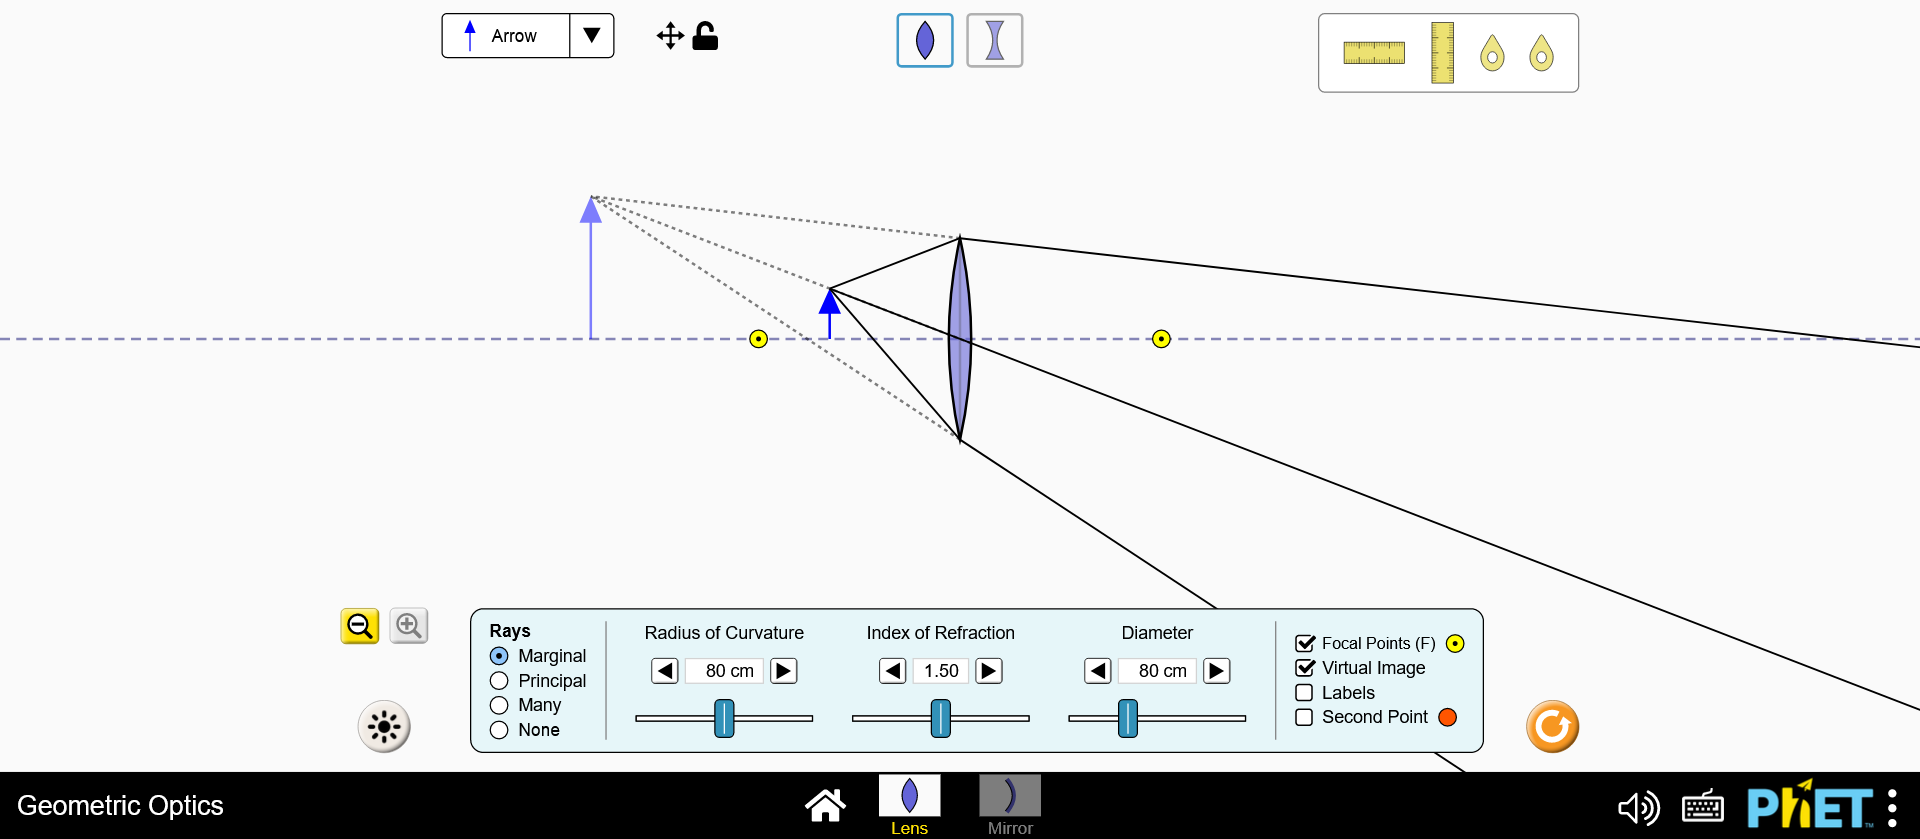
\includegraphics[scale=0.28]{B.png}
	\caption{Ein virtuelles Bild entsteht, wenn die Gegenstandsweite kleiner als die Brennweite der Linse ist.}
\end{figure}

Hier ist zudem erkennbar, dass bei dem reellen Bild Lichtstrahlen vom Bild ausgehen, während vom virtuellen Bild keine Lichtstrahlen ausgehen. 
Die gestrichelten Strahlen sind die imaginären Verlängerungen der nach rechts ausfallenden Lichtstrahlen.
\tiny
Bilder: Geometric Optics version 1.1.1 2022-04-12 23:09:01 UTC PhET Interactive Simuations Copyright © 2002-2022 University of Colorado Boulder \href{https://phet.colorado.edu/sims/html/geometric-optics/latest/geometric-optics_en.html}{->Link}
\normalsize

\section{Abschätzung Brennweite}
\textbf{Wie lässt sich unter Zuhilfenahme der Gaußschen Abbildungsgleichung die Brennweite einer Linse grob abschätzen? Warum ist es dabei von Vorteil, mit einer möglichst großen Gegenstandsweite zu arbeiten?}

Werden die Gegenstandsweite mit $G$, die Bildweite mit $B$, und die Brennweiten der Linse mit $F$ bezeichnet, lautet die Gaußsche Abbildungsgleichung:

$$\frac{1}{B}+\frac{1}{G} = \frac{1}{F}$$

Für große $G$ wird der Term einfacher, weil die Brennweite dann näherungsweise der Bildweite entspricht.

\newpage
\section{Mikroskop}
\textbf{Bitte fertigen sie eine beschriftete Skizze zum Aufbau eines Mikroskops (bestehend aus zwei Linsen) an und erläutern Sie diese kurz.}

\begin{figure}[h]
\centering
	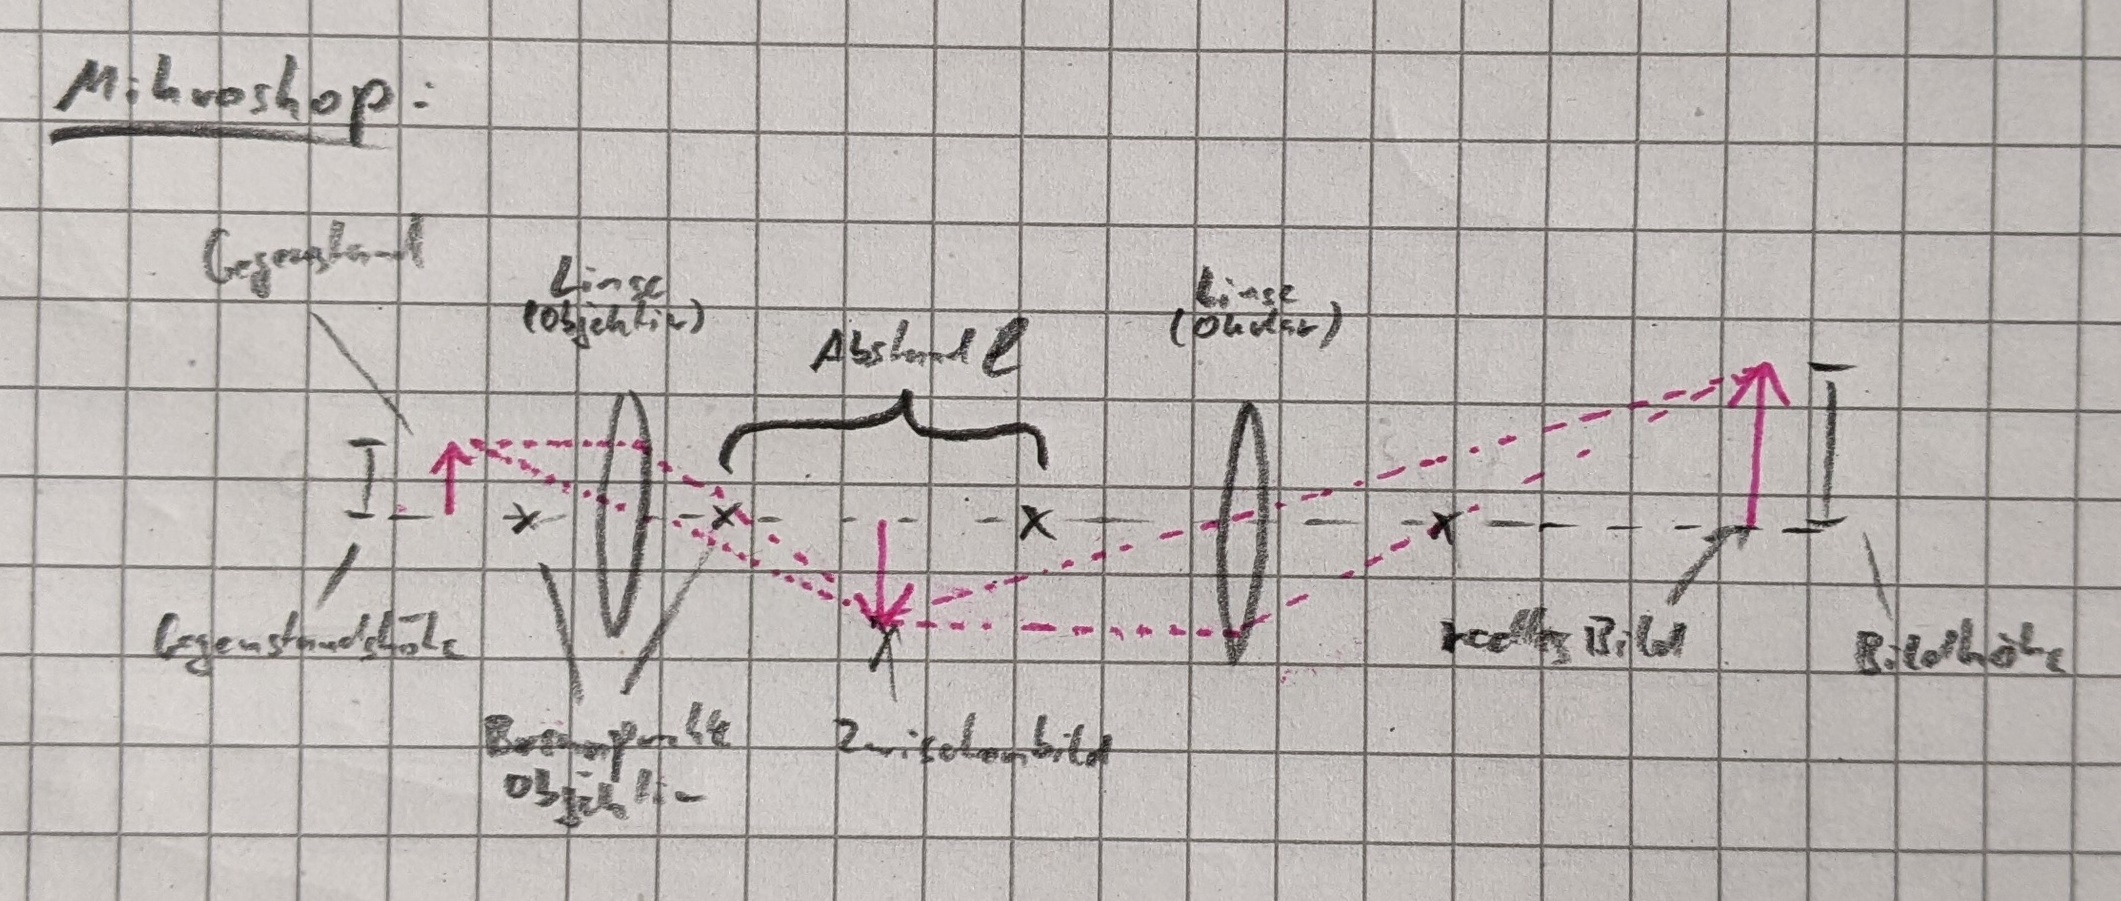
\includegraphics[width=\textwidth]{mikroskop.png}
	\caption{Skizze eines Mikroskopes}
\end{figure}

Das Mikroskop besteht aus zwei Sammellinsen, die im Abstand $l$ voneinander entfernt auf der gleichen optischen Ebene liegen. 
Durch die erste Linse (Objektiv) wird ein Zwischenbild des (sehr) (kleinen) Gegenstandes erstellt.
Durch das Okular wird das entstandene reelle Zwischenbild wie durch eine Lupe nocheinmal vergrößert. 
Das Resultat des Linsensystems ist ein (stark) vergrößertes reelles Bild.
 
\section{Abbe’schen Abbildungstheorie}
\textbf{Unter welcher Bedingung ist die Entstehung eines Bildes im Mikroskop an beugenden Objekten laut der Abbe’schen Abbildungstheorie möglich?}

\begin{figure}[htbp]
\begin{minipage}{0.48\textwidth}
Das beugende Objekt wird solange hinreichend gut abgebildet, wie neben dem Beugungsmaximum 0. Ordnung ein Beugungsmaximum 1. Ordnung von der Apertur des Lichtmikroskopes erfasst wird.
Dafür muss gelten, dass der Winkel $\alpha$ zwischen den Beugungsmaxima und der Gegenstandsebene kleiner ist, als der Winkel $\sigma$ zwischen den vom Objekt aus gesehenen Rändern der Sammellinse.

Durch schräg einfallendes Licht kann erreicht werden, dass das Beugungsmaximum 0. Ordnung nicht im Zentrum der Sammelllinse liegt und somit der Winkel $\alpha$ bis zu doppelt so groß wie der Winkel $\sigma$ sein kann.  

\end{minipage}
\hfill
\begin{minipage}{0.48\textwidth}
	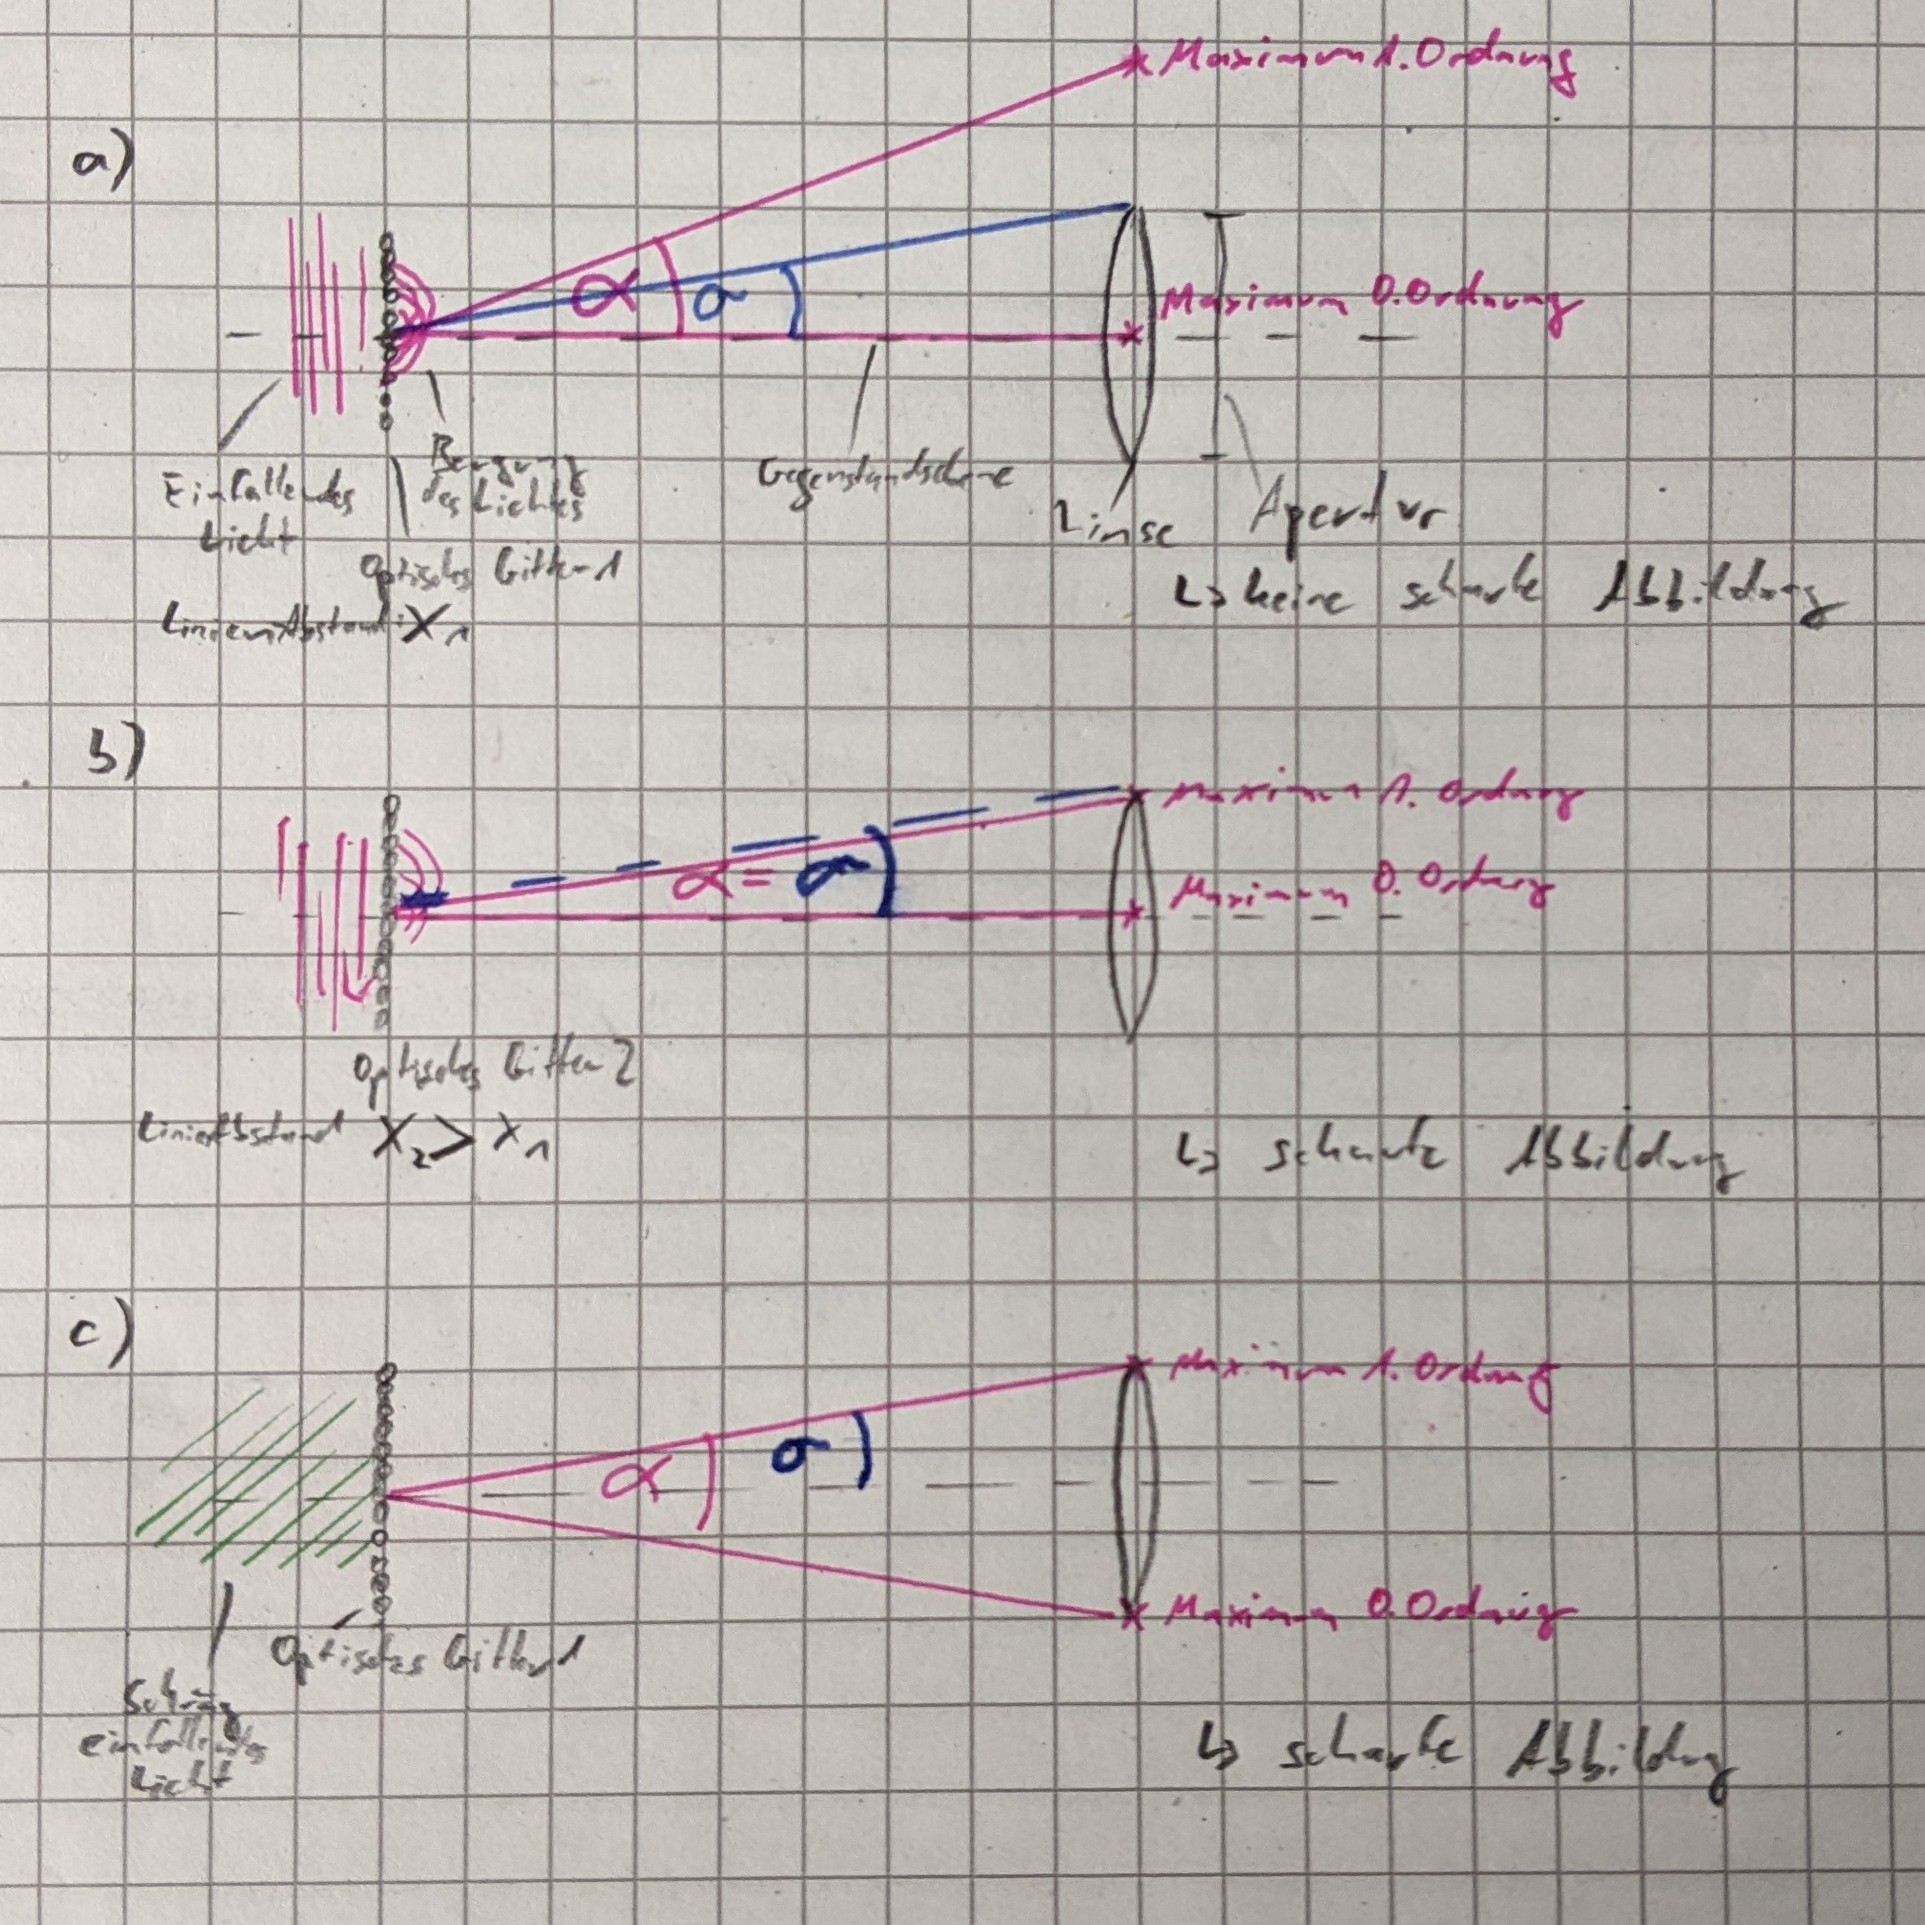
\includegraphics[scale=0.2]{Abbe.png}
\end{minipage}
\end{figure}

Das Kriterium lautet als Formel:
\begin{equation}\label{eq:abbe}
x \geq \frac{\lambda}{A}
\end{equation}

Mit
\begin{itemize}
\item $x$: kleinstmögliche Auflösung
\item $\lambda$: Wellenlänge
\item $A$: Größe Apertur
\end{itemize}

\section{Auflösungsvermögen}
\textbf{Wie verändert sich das Auflösungsvermögen, wenn man die numerische Apertur des Mikroskops vergrößert bzw. verkleinert?}

Wenn die Apertur $A$ größer wird die kleinstmögliche Auflösung $x$ auch kleiner, siehe Gleichung \ref{eq:abbe}.
\end{document}